\documentclass[UTF8,a4paper]{ctexart}

\usepackage{tikz}
\usepackage{multirow}
\usepackage{fontspec}
\usepackage[left=2.50cm, right=2.50cm, top=2.50cm, bottom=2.50cm]{geometry} %页边距
\CTEXsetup[format={\Large\bfseries}]{section} %设置章标题居左
\setmainfont{Courier New}
\setCJKmainfont{阿里巴巴普惠体}

\title{T21 一种组成图的方式}
\author{任凯文}
\pagestyle{empty}

\begin{document}
	\maketitle
	这道题的核心思路是以成语的首尾字为节点,成语为边进行广度优先搜索(bfs),成语的第二、三个字可以不用考虑。下图表示在已知成语为下表中所列的情况下构建的图。选取1,8,9,2和5,233,65,6作为起始和终止节点,那么就将其对应的边从图中删去,并选取2作为广度优先搜索的起点,5作为广度优先搜索的终点,开始搜索并记录下搜索到5时的搜索轮次作为最终答案。
	
	\vspace{.5cm}
	\begin{table}[!hbt]
		\centering
		\begin{tabular}{c}
		\begin{minipage}[b]{.5\linewidth}\begin{tabbing}
			3,89,76,5\hspace{.5cm} \= 4,345,768,5\hspace{.5cm} \= 5,233,65,6 \kill
			1,8,9,2 \> 2,7,6,3 \> 2,12,56,4 \\
			3,89,76,5 \> 4,345,768,5 \> 5,233,65,6
		\end{tabbing}\end{minipage}\\[1em]
		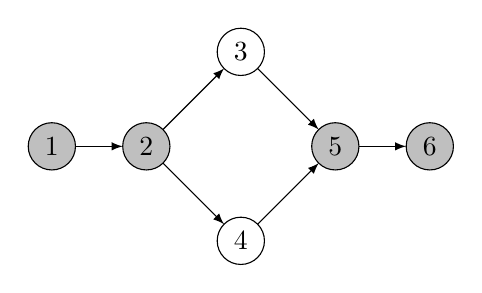
\begin{tikzpicture}[scale=.6]
		\draw[-latex] (-3.5,0) -- (-2.5,0);
		\draw[-latex] (-1.65,0.354) -- (-0.354,1.65);
		\draw[-latex] (-1.65,-0.354) -- (-0.354,-1.65);
		\draw[-latex] (0.354,1.65) -- (1.65,0.354);
		\draw[-latex] (0.354,-1.65) -- (1.65,-0.354);
		\draw[-latex] (2.5,0) -- (3.5,0);
		
		\draw[fill=gray!50] (-4,0)node {1} circle(.5);
		\draw[fill=gray!50] (-2,0)node {2} circle(.5);
		\draw (0,2)node {3} circle(.5);
		\draw (0,-2)node {4} circle(.5);
		\draw[fill=gray!50] (2,0)node {5} circle(.5);
		\draw[fill=gray!50] (4,0)node {6} circle(.5);
		\end{tikzpicture}
	\end{tabular}
	\end{table}
	\vspace{.25cm}
	
	以上是这道题的核心思路,这里要阐述的如何构建图的存储模型。
	
	因为这道题给出输入数据的时候是一行一行地给出的,所以如果想要通过指针构建上图所示的图不仅复杂而且耗时。于是我的做法是通过数组与链表的结合。具体思路如下。
	
	对于每一行输入,只用关注第一个和第四个数据,它们分别对应图中的两个节点(也可能是一个,但是无关紧要)和从第一个节点指向第二个节点的有向边。在此使用一个数组next,next[i]表示值为i的节点可以到达的所有节点,就是以字i为开头的所有成语的结尾。
	
	但是这样成语显然不止一条,而数组的每一位只能储存一个字,那么考虑将每个next的元素作为链表的开头,所有以i为开头的成语的结尾字符均储存在next[i]中即可。
	
	\begin{center}
		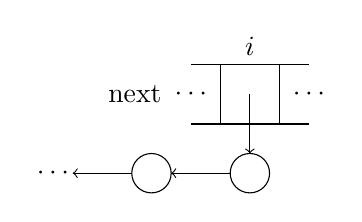
\begin{tikzpicture}[scale=.25]
		\draw (-3,1.5) -- (3,1.5);
		\draw (-3,-1.5) -- (3,-1.5);
		\draw (-1.5,-1.5) rectangle (1.5,1.5);
		\draw (-3,0) node {$\cdots$};
		\draw (-4,0) node[left] {next};
		\draw (3,0) node {$\cdots$};
		\draw (0,1.5) node[above]{$i$};
		
		\draw[->] (0,0) -- (0,-3); \draw(0,-4) circle(1);
		\draw[->] (-1,-4) -- (-4,-4); \draw(-5,-4) circle(1);
		\draw[->] (-6,-4) -- (-9,-4); \draw(-10,-4) node {$\cdots$};
		\end{tikzpicture}
	\end{center}

	在这种情况下如果希望进行搜索,那么选定搜索队列头部的元素,假设为j,将next[j]中的所有链表元素加入队列,然后令该头部元素出队,就完成了一次搜索的步骤。
\end{document}